\documentclass{article}

%\usepackage{fullpage}
\usepackage{booktabs}
\usepackage{graphicx}

\title{Text Mining: Week 6}
\author{Joris van Vugt, s4279859}
\date{\today}

\begin{document}
\maketitle
\section{Introduction}
The goal of the assignment is to create a program for automatic sentiment analysis for tweets. The dataset consists of 110 tweets which contain `\emph{\#Trumph}'. I have manually annotated whether each tweet expresses positive or negative sentiment towards Donald Trump. During annotation I assumed that negative sentiment with respect to Hillary Clinton implies positive sentiment towards Donald Trump. All tweets that did not express any clear sentiment, or were in a language other than English, were discarded. This resulted in 39 tweets with positive sentiment and 39 tweets with negative sentiment towards Trump.

\section{Methods}
I first tried the naive approach of counting the number of positive words and negative words in each tweet using the provided lists of words\footnote{`\emph{Trump}' was removed from the list of positive words for both methods described here}. A tweet containing mostly positive words would be classified as positive and a tweet containing mostly negative words would be classified as negative.
\par
The second approach is tackling the problem with machine learning. First each tweet is preprocessed in the following way: 
\begin{enumerate}
\item All `\texttt{\#}' and `\texttt{@}' symbols are removed.
\item Words that are combined using CamelCase are split (e.g., `\emph{HillaryLiar}' becomes `\emph{Hillary Liar}')
\item Positive words and negative words are replaced with special tokens (resp. `\texttt{<P>}' and `\texttt{<N>}')
\end{enumerate}
All of these steps serve to reduce the size of the vocabulary. After the preprocessing step, a naive Bayes classifier is trained on the \emph{tf-idf} representation of each tweet. Because the training set also has to be predicted, training the model is done using 10-fold cross validation. The model is trained on 9 folds and then predicts the other fold.
\section{Results}
The naive Bayes approach outperformed the word count approach (resp. $F_1=0.46$ and $F_1=0.67$). Therefore, the rest of this section will only discuss the naive Bayes method.

\begin{table}
\centering
\begin{tabular}{llll}
\toprule
\textbf{class} & \textbf{precision} & \textbf{recall} & \textbf{$F_1$-score} \\
\midrule
Positive & 0.68 & 0.64 & 0.66 \\
Negative & 0.66 & 0.69 & 0.68 \\
& & & \\
Average & 0.67 & 0.67 & 0.67 \\
\bottomrule
\end{tabular}
\caption{Performance of the naive Bayes classifier}
\label{tbl:performance}
\end{table}
The hyperparameters yielding the results in Table \ref{tbl:performance} were obtained using grid search. The search space consisted of word, character and word-bound character $n$-grams where $n \in [1, 7]$. Furthermore, each combination was tried with and without preprocessing. This resulted in 42 possible combinations. For each combination, the performance was averaged over 20 runs.
\par Unigrams slightly outperformed character n-grams ($n=4$, $F_1=0.64$). Without the preprocessing steps described earlier the classifier performed worse ($F_1=0.60$). 

\section{Discussion}
I made two considerations during annotating:
\begin{enumerate}
\item \textbf{Tweets that don't directly express sentiment are neutral} \\
A tweet like `\emph{60\% of voters say Hillary beat Trump in debate}' doesn't say anything about the sentiment of the author, so the tweet should not be annotated as positive or negative sentiment.
\item \textbf{Sentiment towards the presidential candidates is mututally exclusive} \\
Negative sentiment with respect to Hillary Clinton implies positive sentiment towards Donald Trump.
\end{enumerate}
Binary classification is a lot easier than multiclass classification, so all neutral tweets were discarded.
\par The mediocre performance can mostly be attributed to the relatively small size of the dataset. After preprocessing, there are still 592 unique words in the the 78 tweets that make up the dataset (682 unqiue words without preprocessing). This results in a very sparse representation of each tweet.

\begin{figure}
\centering
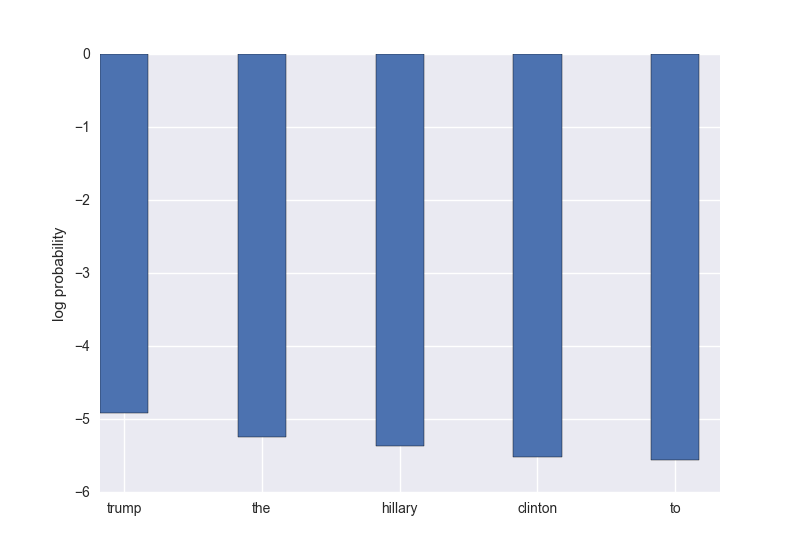
\includegraphics[width=\textwidth]{logprobs.png}
\caption{The terms with the highest probability given positive sentiment with respect to Trump. I.e., $\log p(term|P)$.}
\label{fig:logprobs}
\end{figure}

\section{Conclusion}
Although the performance is better than chance level, I feel like a lot more could be done with more data. I expect bigrams to work better in that case, since a combination of a positive or negative word followed by the name of a presidential candidate can be a very useful feature. Those relations might also be picked up by a more complex classifier (e.g., random forest) using unigrams. Stop word filtering might also be beneficial. Figure \ref{fig:logprobs} shows that if a tweet mentions Hillary Clinton, it is likely to express negative sentiment towards her (i.e., positive sentiment towards Donald Trump). However, stop words (e.g., `\emph{the}' and `\emph{to}') also have relatively high log probabilities. Lastly, given more time, I would also like to add the neutral class.
\end{document}